\documentclass{beamer}
\usepackage{default}
\usepackage{graphicx}				% Use pdf, png, jpg, or eps§ with pdflatex; use eps in DVI mode
% TeX will automatically convert eps --> pdf in pdflatex
\usepackage{amssymb}
\usepackage{amsmath}
\usepackage{algpseudocode}% http://ctan.org/pkg/algorithmicx
\usepackage{mathtools,xparse}
\usepackage{dsfont}
\usepackage[]{algorithm2e}

\DeclareMathOperator*{\argmin}{\arg\!\min}
\DeclareMathOperator*{\argmax}{\arg\!\max}
\SetKwProg{Fn}{Function}{}{}

\title{Probabilistic Logic and Deep Learning\\
\large Timothy Zhang\\
Stony Brook University\\
Research Proficiency Examination}
\date{}							% Activate to display a given date or no date

\begin{document}
	\maketitle
	
\begin{frame}
	\frametitle{Agenda}
	\begin{itemize}
		\item \textbf{Deep Learning}
		\item Logical Student-Teacher Network
		\item Probabilistic Logic Programming
		\item TensorLog
		\item Conclusion
	\end{itemize}
\end{frame}

\begin{frame}
\frametitle{Deep Neural Networks}
\begin{figure}
	\begin{center}
		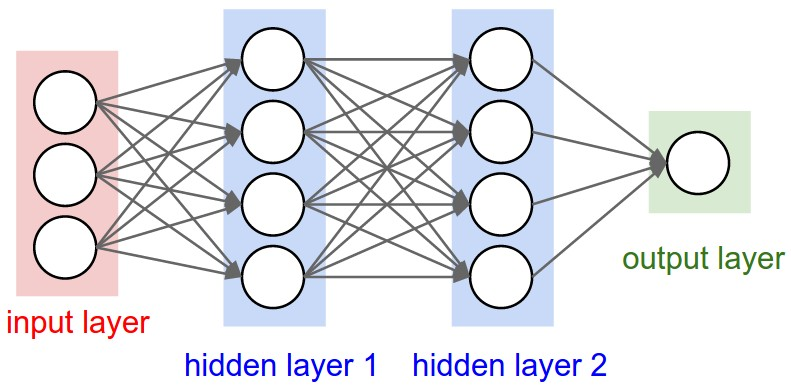
\includegraphics[width=8cm, height=4cm]{dnn}
	\end{center}
	\caption{A two layer neural network $g(\textbf{x}) = o(h_2(h_1(x)))$.}
\end{figure}
\begin{itemize}
	\item $\textbf{x} \in \mathbb{R}^3$, $\textbf{y} \in \mathbb{R}$
	\item $h_1(\textbf{x}) = \phi_1(W_1 \textbf{x} + b_1)$
	\item $h_2(h_1(\textbf{x})) = \phi_2(W_2 h_1(\textbf{x}) + b_2)$
	\item $o(h_2(h_1(\textbf{x}))) = \psi(W_3 \phi_2(\phi_1(\textbf{x})) + b_3)$
\end{itemize}
\end{frame}

\begin{frame}
\frametitle{Deep Neural Networks}
\begin{figure}
	\begin{center}
		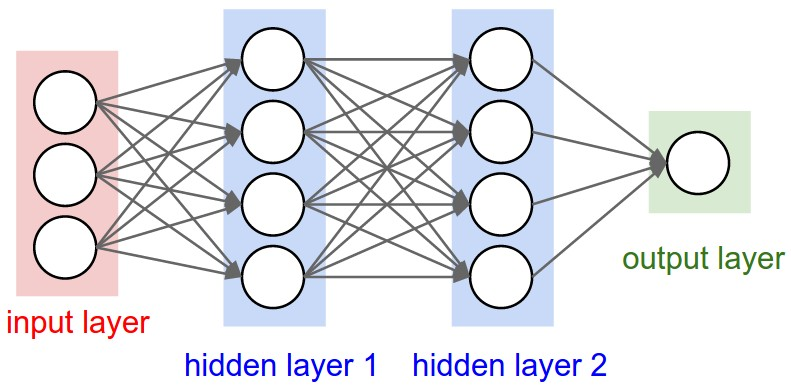
\includegraphics[width=8cm, height=4cm]{dnn}
	\end{center}
	\caption{A two layer neural network $g(\textbf{x}) = o(h_2(h_1(x)))$.}
\end{figure}
\begin{itemize}
	\item Each $\phi_i$ is a nonlinear function applied element-wise to the hidden layer output.
	\item Ex: tanh, ReLu, logistic sigmoid
	\item $\psi_j$ is a function applied to the output layer output.
	\item Ex: identity, softmax
\end{itemize}
\end{frame}

\begin{frame}
\frametitle{Deep Neural Networks}
\begin{figure}
	\begin{center}
		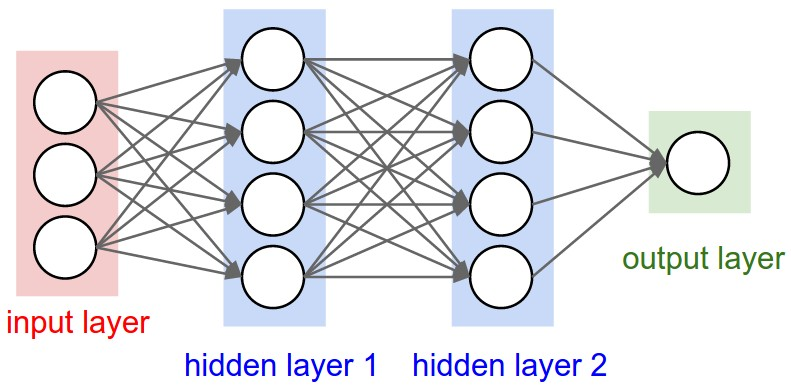
\includegraphics[width=8cm, height=4cm]{dnn}
	\end{center}
	\caption{A two layer neural network $g(\textbf{x}) = o(h_2(h_1(x)))$.}
\end{figure}
\begin{itemize}
	\item A loss (objective, reward, etc) function is defined with respect to the output of the network and the ground truth label.
	\item Ex: MSE is $\sum_i (\textbf{y}^{(i)} - g(\textbf{x}^{(i)}))^2$
\end{itemize}
\end{frame}

\begin{frame}
\frametitle{Deep Neural Networks}
	\begin{algorithm}[H]
	\KwData{
		Training data $\mathcal{S} = \{(\textbf{x}^{(n)}, \textbf{y}^{(n)})\}_{n = 1}^{N}$,\\
		\hspace*{1.15cm} Hyperparameters: $\eta$ learning rate
	}
	\KwResult{$\boldsymbol{\theta}^*$ which minimizes $\mathcal{L}$\newline}
	Initialize DNN parameters $\boldsymbol{\theta}$ \\
	\While{$\lnot$ converged}{
		Sample a minibatch $(X, Y) \subset \mathcal{S}$ \\
		Set $g \leftarrow 0$ \\
		\For{$(\textbf{x}, \textbf{y}) \in (X, Y)$}{
			Compute gradient: $g \leftarrow g + \nabla_\theta \mathcal{L}(f_\theta(\textbf{x}), \textbf{y}; \boldsymbol{\theta})$
		}
		Apply update: $\boldsymbol{\theta} \leftarrow \boldsymbol{\theta} - \eta g$
	}
	\caption{Stochastic Gradient Descent}
\end{algorithm}
\end{frame}

\begin{frame}
\frametitle{Agenda}
\begin{itemize}
	\item Deep Learning
	\item \textbf{Logical Student-Teacher Network}
	\item Probabilistic Logic Programming
	\item TensorLog
	\item Conclusion
\end{itemize}
\end{frame}

\begin{frame}
	\frametitle{Architecture}
	\begin{figure}
		\begin{center}
			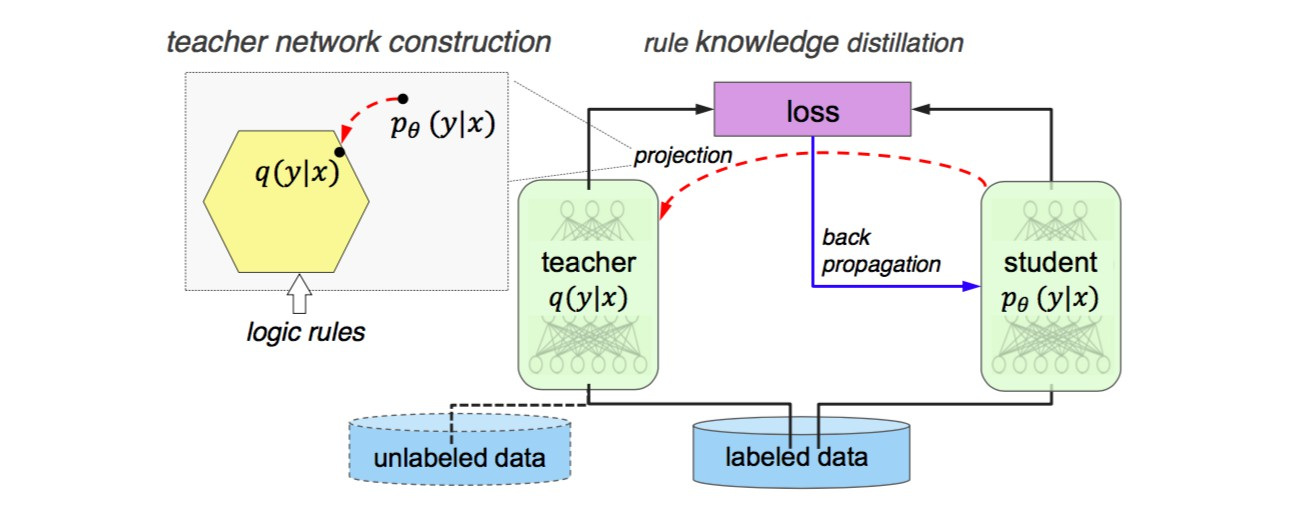
\includegraphics[width=12cm, height=5.5cm]{teacher_dnn}
		\end{center}
	\end{figure}
\end{frame}

\begin{frame}
\frametitle{Loss Function}
\begin{figure}
	\begin{center}
		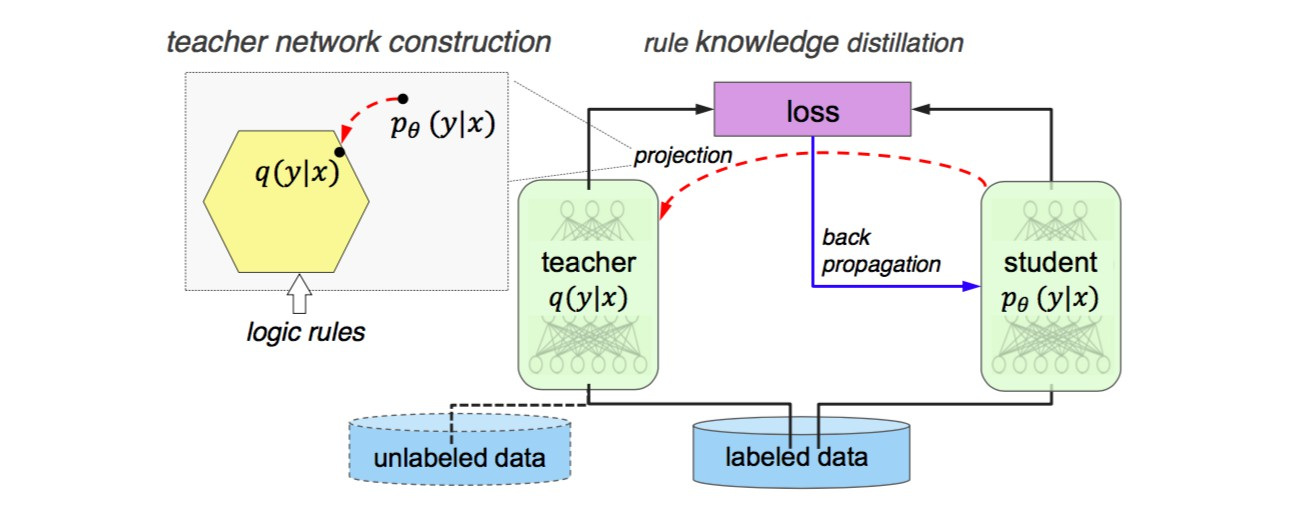
\includegraphics[width=6.5cm, height=3cm]{teacher_dnn}
	\end{center}
\end{figure}
\begin{equation}
\boldsymbol{\theta}^{(t + 1)} = \argmin_{\theta \in \Theta} \frac{1}{N} \sum_{n = 1}^{N} (1 - \pi) \mathcal{L}(\textbf{y}_n, \boldsymbol{\sigma}_{\theta}(\textbf{x}_{n})) + \pi \mathcal{L}(s_n^{(t)}, \boldsymbol{\sigma}_{\theta}(\textbf{x}_n))
\end{equation}
\begin{itemize}
	\item  $\textbf{x}_n, \textbf{y}_n$: $nth$ sample
	\item $\mathcal{L}$ is an arbitrary loss (assume cross-entropy)
	\item $\pi$ is the mixture weight between student and teacher networks
	\item $\boldsymbol{\sigma}_{\theta}(\textbf{x}_n)$ is the output from the student network (assumed to be a softmax vector)
	\item $s_n^{(t)}$: teacher network output at iteration $t$
\end{itemize}
\end{frame}

\begin{frame}
\frametitle{Logic Rules}
\begin{itemize}
\item $\mathcal{R} = \{(R_l, \lambda_l) \}_{l = 1}^L$ where each $R_l$ is a first-order logic formula with an associated confidence $\lambda_l \in [0, \infty]$.
\item These rules are encoded using a continuous logic called soft logic which allows continuous truth values $\in [0, 1]$ with the following semantics:
\end{itemize}

\begin{equation}
\begin{gathered}
\neg A = 1 - A\\
A \& B = \max\{A + B - 1, 0\}\\
A \lor B = \min\{A + B, 1\}\\
A_1 \land ... \land A_N = \sum_i A_i / N
\end{gathered}
\end{equation}
\end{frame}

\begin{frame}
\frametitle{Teacher Network Construction}
\framesubtitle{Loss function}
\begin{equation}
\begin{gathered}
\min_{q, \xi \geq 0}  \text{KL}(q(Y|X) || p_\theta(Y|X)) + C \sum_{l, g_l} \xi_{l, g_l}\\
\text{s.t. } \lambda_l (1 - \mathbf{E}_q[r_{l,g_l}(X, Y)]) \leq \xi_{l, g_l}\\
g_l = 1,...,G_l, l= 1,..., L.
\end{gathered}
\end{equation}

\begin{itemize}
\item Intuitively, we want the teacher network distribution $q$ to be close to the student network $p_\theta$, so we use a KL term. 
\item Additionally we want the soft logic rules to approximately hold, so we use an expectation term in the constraints and introduce slack variables $\xi$.
\end{itemize}
\end{frame}

\begin{frame}
\frametitle{Teacher Network Construction}
\framesubtitle{Dual Lagrangian}
Rewrite (3) in standard form.
\begin{gather*}
\min_{q, \xi} \text{KL}(q(Y|X) || p_\theta(Y|X)) + C \sum_{l, g_l} \xi_{l, g_l}\\
\text{s.t. } \lambda_l (1 - \mathbf{E}_q[r_{l,g_l}(X, Y)]) - \xi_{l, g_l}\leq 0\\
-\xi_{l, g_l} \leq 0\\
\sum_Y q(Y|X) - 1 = 0\\
g_l = 1,...,G_l, l= 1,..., L
\end{gather*}
Then add Lagrange multipliers and simplify (algebra)
\begin{gather*}
\max_{\eta \geq 0, \mu \geq 0, \alpha \geq 0} \min_{q, \xi}  \text{KL}(q(Y|X) || p_\theta(Y|X)) + C \sum_{l, g_l}  \xi_{l, g_l} \\
+ \sum_{l, g_l} \eta_{l, g_l}(\mathbf{E}_q[\lambda_l (1 - r_{l, g_l}(X, Y))] - \xi_{l, g_l}) - \sum_{l, g_l} \mu_{l, g_l}   \xi_{l, g_l} + \alpha(\sum_Y q(Y|X) - 1).
\end{gather*}
\end{frame}

\begin{frame}
\frametitle{Teacher Network Construction}
\framesubtitle{Teacher Construction Rule}
By solving the dual Lagrangian we obtain the teacher network construction rule:
\begin{gather}
q^*(Y|X) \propto p_\theta(Y|X) \exp\bigg \{ -\sum_{l,g_l}C \lambda_l (1 - r_{l,g_l}(X, Y)) \bigg \}.
\end{gather}
\begin{itemize}
	\item $q^*(Y|X)$ can be computed efficiently for a given example $\textbf{x}$
	\item We simply feed $\textbf{x}$ as input to the student network and use the output vector $\boldsymbol{\sigma}_{\theta}(\textbf{x})$ as $p_\theta(Y|X)$ in the above expression.
	\item Thus an inference step in the teacher network will have complexity of the order $O(lg_l + \mathcal{I})$ where $ \mathcal{I}$ is the complexity of inference in the student network.
\end{itemize}
\end{frame}

\begin{frame}
\frametitle{Learning Algorithm}
\begin{algorithm}[H]
\KwData{
Training data $\mathcal{S} = \{(\textbf{x}_n, \textbf{y}_n)\}_{n = 1}^{N}$,\\
\hspace*{1.15cm} Rule set $\mathcal{R} = \{(R_l, \lambda_l)\}_{l = 1}^L$,\\
\hspace*{1.15cm} Hyperparameters: $\pi$ imitation parameter,\\
\hspace*{4cm} $C$ regularization strength
}
\KwResult{Trained networks $p_\theta$ and $q$\newline}
Initialize DNN parameters $\boldsymbol{\theta}$ \\
\While{$\lnot$ converged}{
Sample a minibatch $(X, Y) \subset \mathcal{S}$ \\
Construct teacher network $q$ using (4)\\
Update $\boldsymbol{\theta}$ using (1) \\
}
\caption{Teacher and Student Network Training}
\end{algorithm}
\end{frame}

\begin{frame}
\frametitle{Sentence Level Sentiment Analysis}
\framesubtitle{Student Network Architecture}
\begin{figure}
\begin{center}
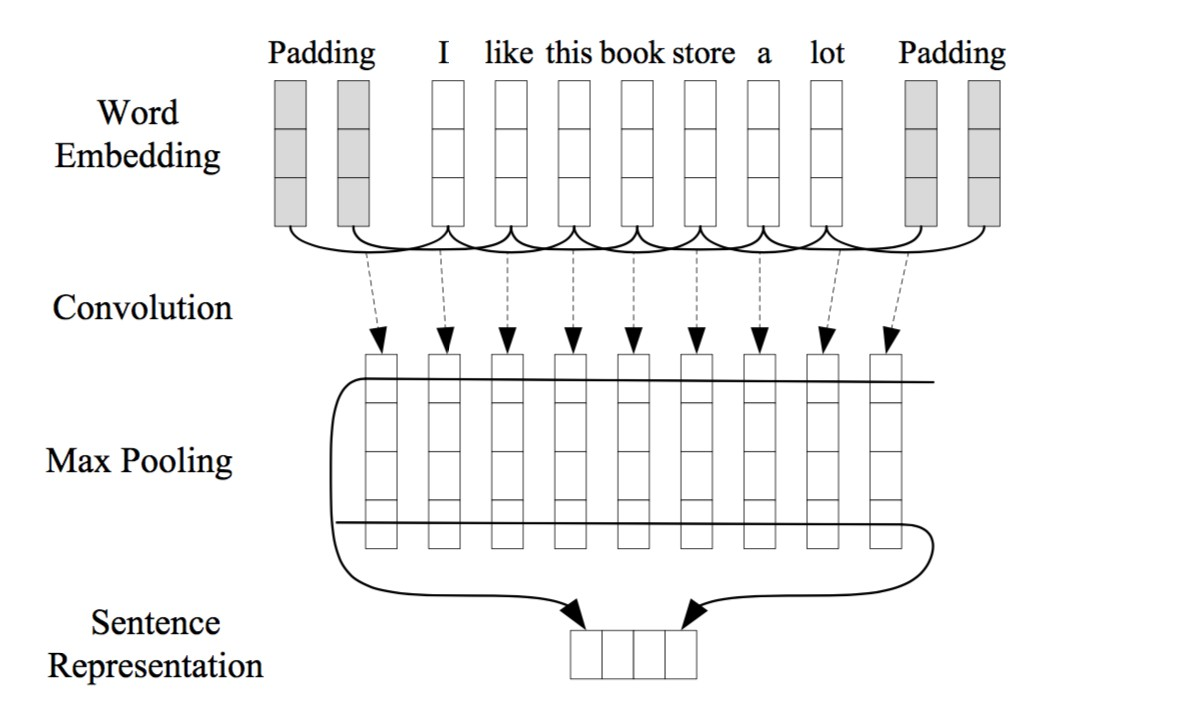
\includegraphics[width=12cm, height=6cm]{cnn}
\caption{CNN architecture using Word2Vec vectors.}
\end{center}
\end{figure}
\end{frame}

\begin{frame}
\frametitle{Sentence Level Sentiment Analysis}
\framesubtitle{Logic Rule}
\begin{gather*}
\text{has-A-but-B-structure}(S) \Rightarrow \\
(\mathbf{1}(y = +) \Rightarrow \boldsymbol{\sigma}_\theta(B)_+ \land \boldsymbol{\sigma}_\theta(B)_+ \Rightarrow \mathbf{1}(y = +)),
\end{gather*}
\begin{itemize}
\item Intuitively, if a sentence has a "but" in it we should take the sentiment of the subsentence after the "but".
\item ``At first I thought the movie was great but it turned out to be derivative and boring."
\end{itemize}
\end{frame}

\begin{frame}
\frametitle{Sentence Level Sentiment Analysis}
\framesubtitle{Results}
\begin{figure}
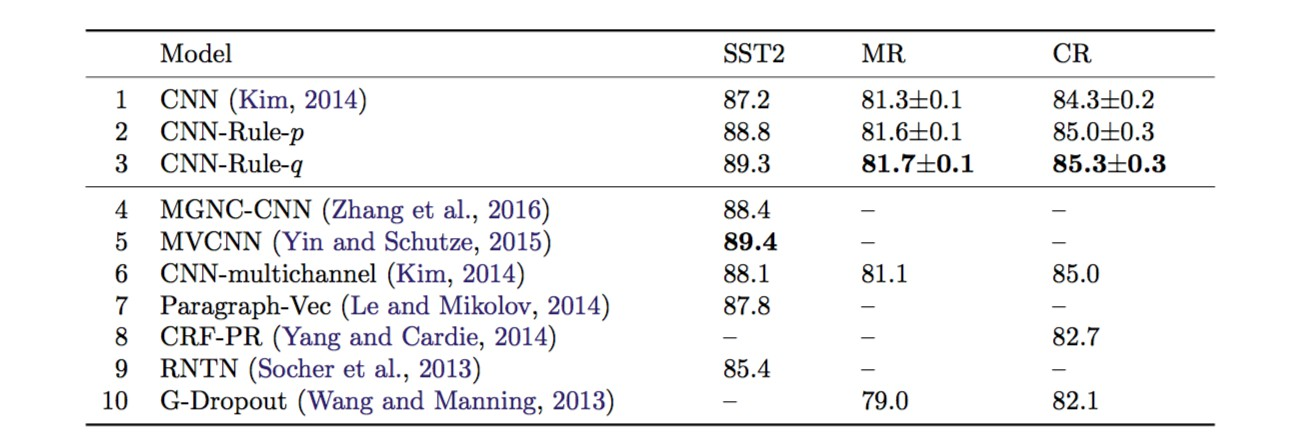
\includegraphics[width=11.5cm, height=4.5cm]{cnn_results}
\end{figure}
\end{frame}

\begin{frame}
\frametitle{Agenda}
\begin{itemize}
	\item Deep Learning
	\item Logical Student-Teacher Network
	\item \textbf{Probabilistic Logic Programming}
	\item TensorLog
	\item Conclusion
\end{itemize}
\end{frame}


\begin{frame}
\frametitle{Agenda}
\begin{itemize}
	\item Deep Learning
	\item Logical Student-Teacher Network
	\item Probabilistic Logic Programming
	\item \textbf{TensorLog}
	\item Conclusion
\end{itemize}
\end{frame}

\begin{frame}
\frametitle{Logical Inference and Neural Networks}
\begin{itemize}
	\item Logical specifications allow one to model aspects of the world and perform \textbf{logical inference}.
	\item In Prolog this is done using SLD-resolution, which is a search procedure over proofs for a query.
	\item Discrete search is not a differentiable function, and thus cannot directly be integrated in gradient-based learning systems.
\end{itemize}
\end{frame}

\begin{frame}
\frametitle{TensorLog}
\begin{itemize}
	\item TensorLog proposes a differentiable (probabilistic) logical inference procedure.
	\item This algorithm can be seen as an instance of the Belief Propagation algorithm for probabilistic graphical models.
	\item Thus TensorLog offers a method of incorporating traditional logical inference as a component of a DNN.
	\item Alternatively, TensorLog offers a method of incorporating DNNs for traditional logical inference.
\end{itemize}
\end{frame}

\begin{frame}[fragile]
\frametitle{Example TensorLog Model}
\begin{figure}
	\begin{center}
		\begin{verbatim}
		% Theory T
		uncle(X, Y) :- child(X, Z), brother(Z, Y).
		uncle(X, Y) :- aunt(X, W), husband(W, Y).
		status(X, tired) :- child(W, X), infant(W).
		
		% Knowledge Base DB
		0.99 :: child(liam, eve).     0.7 :: infant(liam).
		0.99 :: child(dave, eve).     0.1 :: infant(dave).
		0.75 :: child(liam, bob).     0.9 :: aunt(joe, eve).
		0.9 :: husband(eve, bob).     0.9 :: brother(eve, chip).
		\end{verbatim}
	\end{center}
	\caption{Example $\mathcal{DB}$ and $\mathcal{T}$.}
\end{figure}
\end{frame}

\begin{frame}
\frametitle{Logical Preliminaries}
\begin{itemize}
	\item A \textbf{database} $\mathcal{DB} = \{f_1, ..., f_N \}$ where each $f_i$ is a ground \textbf{fact}.
	\item A fact is of the form $p(a, b)$ or $q(c)$ where $p$ and $q$ are predicate symbols and $a, b, c \in \mathcal{C}$ are constant symbols from domain $\mathcal{C}$.
	\item A theory $\mathcal{T}$, is a set
	of function-free Horn clauses.
	\item The least model for $(\mathcal{DB}, \mathcal{T})$ is written $Model(\mathcal{DB}, \mathcal{T})$.
	\item A fact $f$ is true iff $f \in Model(\mathcal{DB}, \mathcal{T})$
\end{itemize}
\end{frame}

\begin{frame}
\frametitle{Probabilistic Logical Preliminaries}
\begin{itemize}
	\item $\Theta$ is a parameter vector over the facts $f \in \mathcal{DB}$ s.t. $\theta_f \in [0,1]$.
	\item The semantics of this parameter
	vary in different probabilistic deductive database models
	\item $\Theta$ defines a distribution $Pr(f | \mathcal{T}, \mathcal{DB}, \Theta)$ over facts in $Model(\mathcal{T}, \mathcal{DB})$.
\end{itemize}
\end{frame}

\begin{frame}
\frametitle{TensorLog Logical Restrictions}
\begin{itemize}
	\item TensorLog is function free.
	\item Predicates in TensorLog have arity at most 2.
	\item Queries are of the form $q(a, X) \leftarrow b_1(a, c), ..., b_k(z, b).$ or $q(X, b) \leftarrow b_1(a, c), ..., b_k(z, b).$
	\item Thus we are interested in all relationships between some constant $a$ and all other constants $b$ s.t. $q(a, X)[X/b]$ holds in the theory.
	\item TensorLog only models restricted Datalog programs of this form and does so using matrix representations of predicates and constants.
\end{itemize}
\end{frame}

\begin{frame}
\frametitle{TensorLog Matrix Representation}
\begin{itemize}
	\item It is assumed that there is some arbitrary order on $c \in C$ corresponding to indices $[1, ..., |C|]$ which holds in all matrices and vectors.
	\item Constants $c \in C$ are represented using a one-hot row-vector $\textbf{u} \in \mathbf{R}^{|C|}$.
	\item Binary predicates are represented as a sparse matrix $\textbf{M}_r$ where $\textbf{M}_r[i, j] = \theta_{r(i, j)}$ if $r(i, j) \in \mathcal{DB}$, and 0 otherwise.
	\item  A unary predicate $q$ is represented analogously as a row-vector $\textbf{v}_q$.
\end{itemize}
\end{frame}

\begin{frame}[fragile]
\frametitle{TensorLog Matrix Representation Example}
\begin{figure}
	\begin{center}
		\begin{verbatim}
		% Knowledge Base DB
		0.99 :: child(liam, eve).     0.7 :: infant(liam).
		0.99 :: child(dave, eve).     0.1 :: infant(dave).
		0.75 :: child(liam, bob).     0.9 :: aunt(joe, eve).
		0.9 :: husband(eve, bob).     0.9 :: brother(eve, chip).
		\end{verbatim}
	\end{center}
\end{figure}
When the order is $[liam, eve, dave, bob, joe, chip]$, 
$\textbf{M}_{child}
= 
\begin{bmatrix}
\theta_{child(liam, liam)} & \theta_{child(liam, eve)}  & ...  & \theta_{child(liam, chip)} \\
\theta_{child(eve, liam)} & \theta_{child(eve, eve)}  & ... & \theta_{child(eve, chip)} \\
\hdotsfor{4} \\

\theta_{child(chip, liam)} & \theta_{child(chip, eve)}  & ... & \theta_{child(chip, chip)} \\
\end{bmatrix} $
\linebreak \linebreak
$\textbf{v}_{infant}
= 
\begin{bmatrix}
0.7 & 0 & 0.1 &0&0&0
\end{bmatrix} $
\newline\newline
We will use matrix multiplication to implement logical inference.
\end{frame}

\begin{frame}
\frametitle{Probabilistic Graphical Models I}
\begin{itemize}
	\item A probabilistic graphical model (PGM) represents the joint probability distribution of a set of random variables $Pr(X)$.
	\item Naively the joint factorizes as $Pr(X = x_1, x_2, ..., x_n) =  Pr(x_1) \times Pr(x_2 | x_1) \times ... \times Pr(x_n | x_{n-1}, x_{n -2 }, ..., x_2, x_1)$
	\item Generally, we want factorizations which minimize the number of parameters.  We achieve this by introducing conditional independence relations.
	\item Ex: Bayesian networks (directed graphical models) encode the factorization as \begin{gather*}
	p(X) = \prod_{i} p(x_i | \pi(x_i))
	\end{gather*}
	where $\pi(x) = \{ x' : (x', x) \in E \}$.
\end{itemize}
\end{frame}

\begin{frame}
\frametitle{Probabilistic Graphical Models II}
\begin{figure}
	\begin{center}
		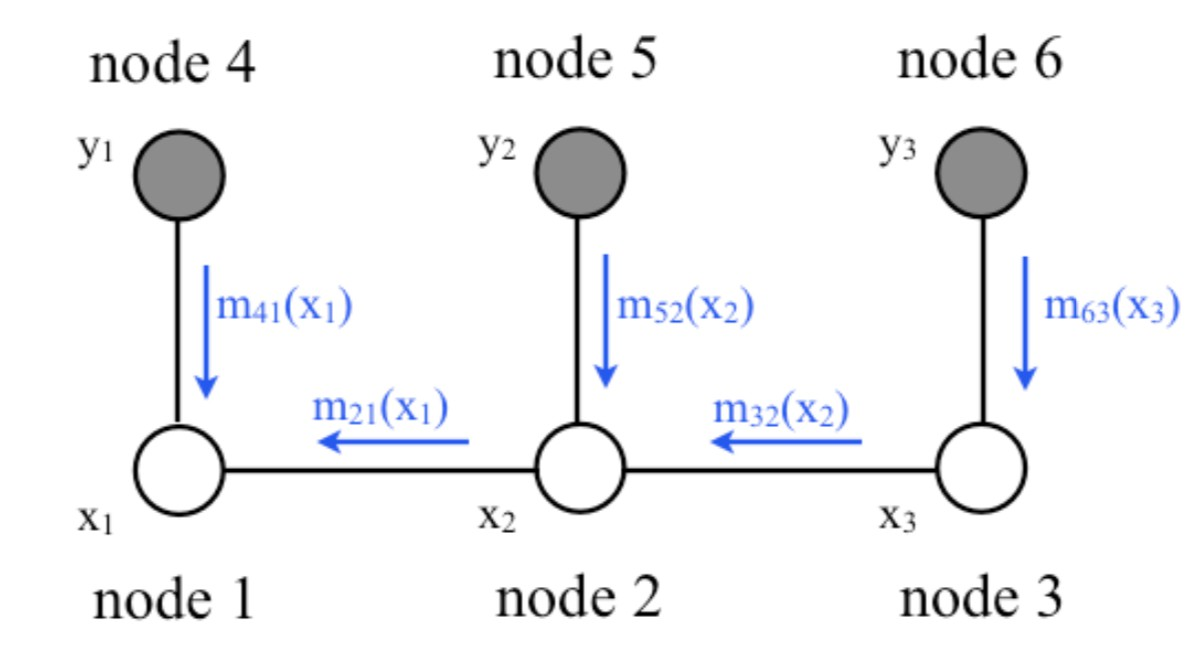
\includegraphics[width=8cm, height=4cm]{bp}
	\end{center}
\end{figure}
Markov chain with three observed variables $y_1, y_2, y_3$ and three hidden variables $x_1, x_2, x_3$.  The factorization of this example is: 
\begin{gather*}
p(X, Y) = \frac{1}{Z} \psi_{12}(x_1, x_2) \psi_{23}(x_2, x_3) \phi_1(x_1, y_1) \phi_2(x_2, y_2) \phi_3(x_3, y_3).
\end{gather*}
\end{frame}

\begin{frame}
\frametitle{Probabilistic Graphical Models III}
\begin{figure}
	\begin{center}
		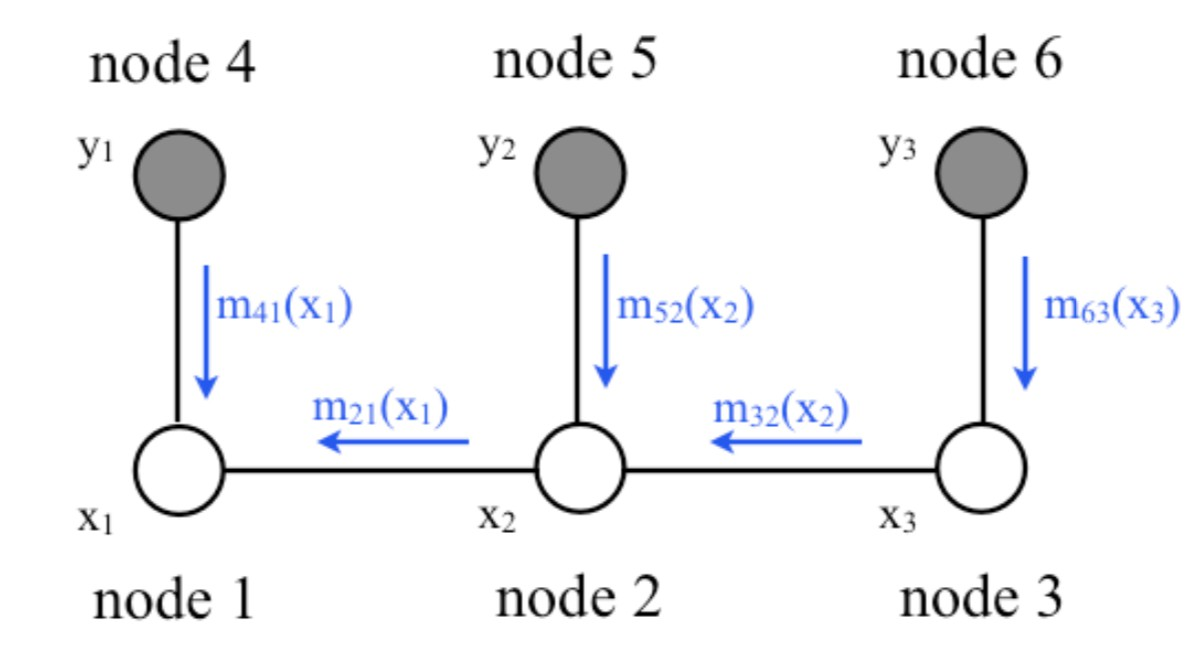
\includegraphics[width=4.5cm, height=2cm]{bp}
	\end{center}
\end{figure}
\begin{itemize}
	\item In practice we will be interested in using a PGM to perform inference over some subset of the random variables; ie. computing the probability of the subset $p(X' \subseteq X)$. 
	\item Assume that we wish to compute the marginal probability of $x_1$ given $Y$: 
	\begin{gather*}
	p(x_1 | Y) = \frac{1}{p(Y)} \sum_{X_2} \sum_{X_3} p(X, Y),
	\end{gather*}
	where the equation is due to the fact that $p(X|Y) = \frac{p(X,Y)}{p(Y)}$.
\end{itemize}
\end{frame}

\begin{frame}
\frametitle{Belief Propagation I}
\begin{figure}
	\begin{center}
		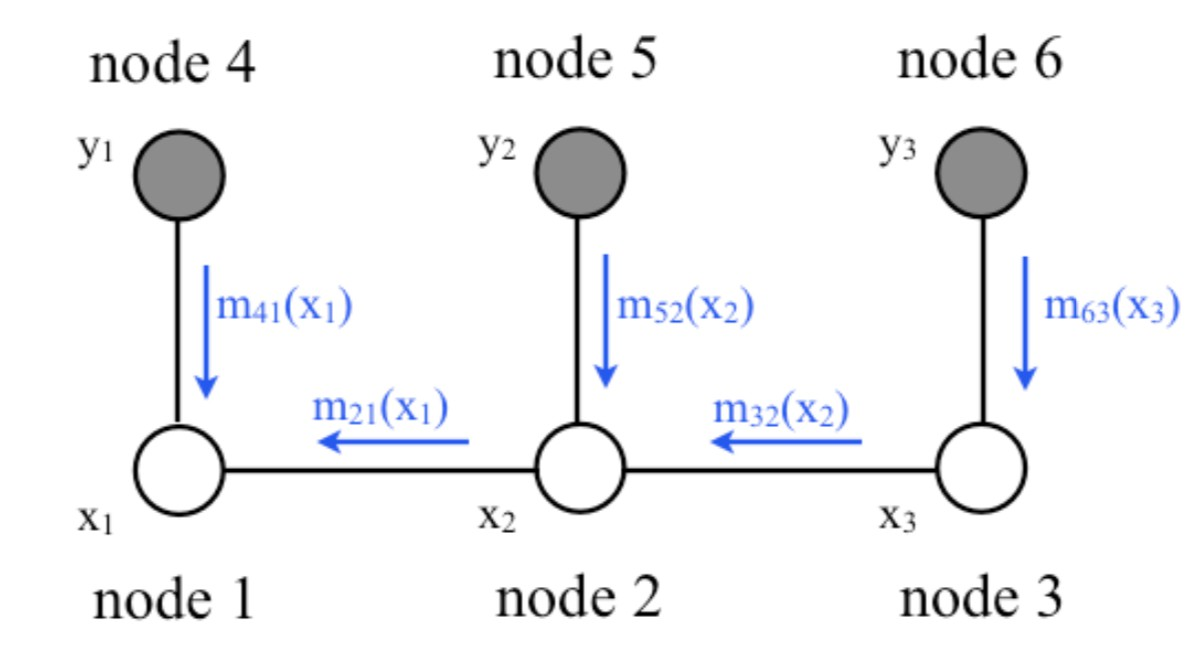
\includegraphics[width=6.5cm, height=3.15cm]{bp}
	\end{center}
\end{figure}
\begin{gather*}
p(x_1 | Y) = \frac{1}{p(Y)} \sum_{X_2} \sum_{X_3} p(X, Y)\\
= \frac{1}{p(Y)} \sum_{X_2} \sum_{X_3} \psi_{12}(x_1, x_2) \psi_{23}(x_2, x_3) \phi_1(x_1, y_1) \phi_2(x_2, y_2) \phi_3(x_3, y_3).\\
= \frac{1}{p(Y)} \phi_1(X_1, y_1) \sum_{X_2 = x_2} \psi_{12}(X_1, x_2) \phi_2(x_2, y_2) \sum_{X_3 = x_3} \psi_{23}(x_2, x_3) \phi_3(x_3, y_3)\\
= \frac{1}{p(Y)} m_{41}(x_1) \sum_{X_2 = x_2} \psi_{12}(X_1, x_2) m_{52}(x_2) \sum_{X_3 = x_3} \psi_{23}(x_2, x_3) m_{63}(x_3)
\end{gather*}
\end{frame}

\begin{frame}
\frametitle{Belief Propagation II}
\begin{figure}
	\begin{center}
		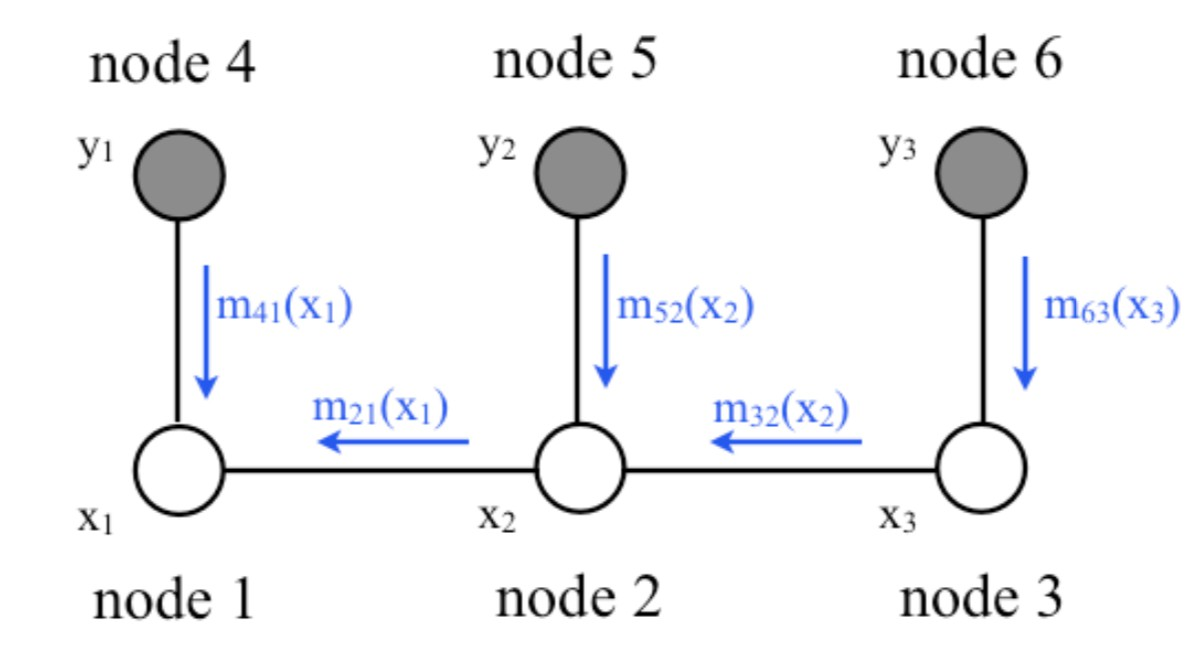
\includegraphics[width=6.5cm, height=3cm]{bp}
	\end{center}
\end{figure}
\begin{gather*}
\frac{1}{p(Y)} m_{41}(x_1) \sum_{X_2 = x_2} \psi_{12}(X_1, x_2) m_{52}(x_2) \sum_{X_3 = x_3} \psi_{23}(x_2, x_3) m_{63}(x_3)
\end{gather*}
Let's take a closer look at these messages.
\begin{itemize}
	\item $m_{41}(x_1) = \phi_1(x_1, y_1)$
	\item $m_{52}(x_2) = \phi_2(x_2, y_2)$
	\item $m_{63}(x_3) = \phi_3(x_3, y_3)$
\end{itemize}
All of these messages are scalars which are known.
\end{frame}

\begin{frame}
\frametitle{Belief Propagation III}
\begin{figure}
	\begin{center}
		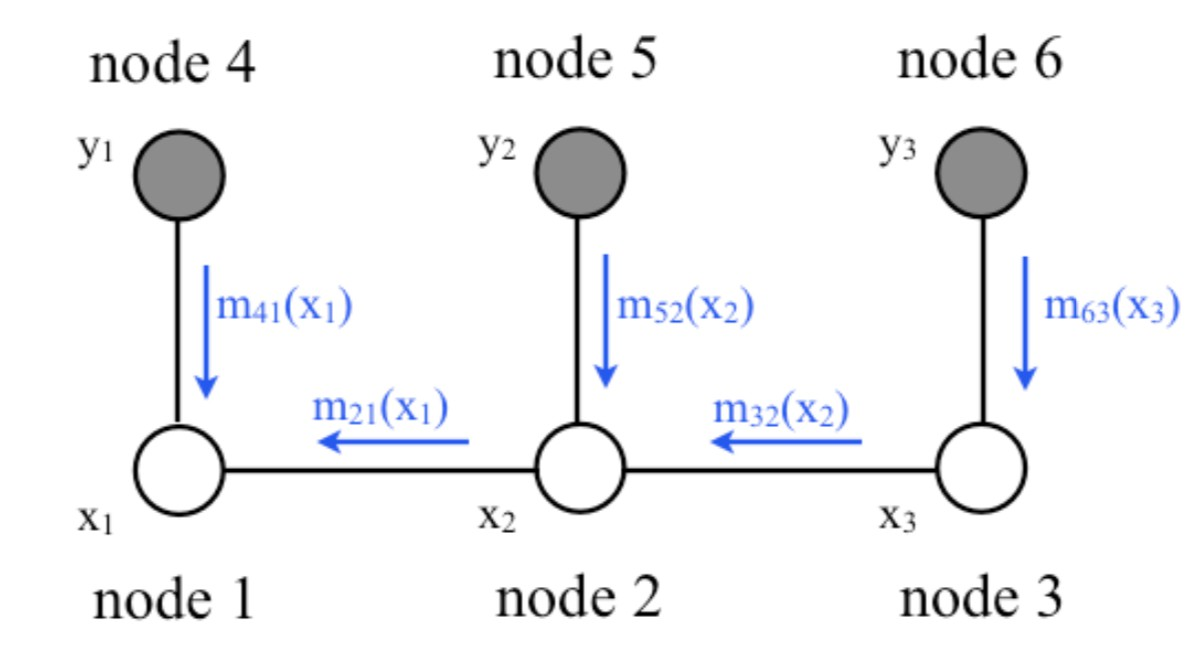
\includegraphics[width=6.5cm, height=3cm]{bp}
	\end{center}
\end{figure}
\begin{gather*}
\frac{1}{p(Y)} m_{41}(x_1) \sum_{X_2 = x_2} \psi_{12}(X_1, x_2) m_{52}(x_2) \sum_{X_3 = x_3} \psi_{23}(x_2, x_3) m_{63}(x_3)\\
= \frac{1}{p(Y)} m_{41}(x_1) \sum_{X_2 = x_2} \psi_{12}(X_1, x_2) m_{52}(x_2) m_{32}(x_2)\\
= \frac{1}{p(Y)} m_{41}(x_1) m_{21}(x_1).
\end{gather*}
Finally, if we were to compute say $p(x_2 | Y)$ we would be able to reuse many of these messages.
\end{frame}

\begin{frame}
\frametitle{Belief Propagation IV}
\begin{figure}
	\begin{center}
		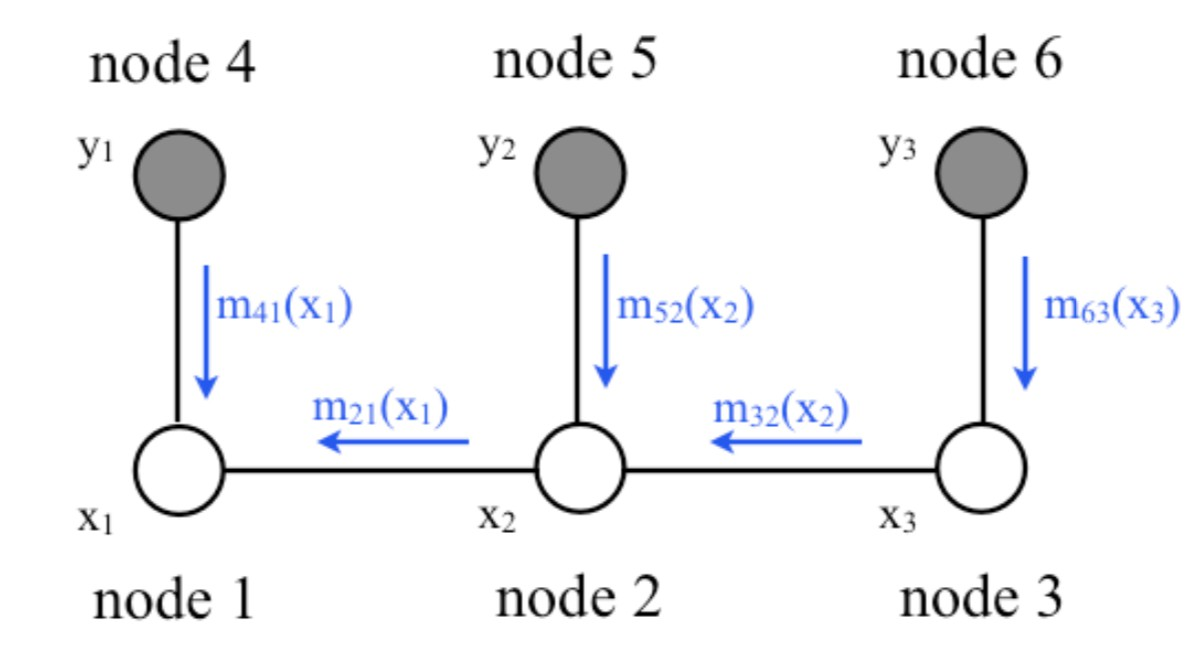
\includegraphics[width=6.5cm, height=3cm]{bp}
	\end{center}
\end{figure}
\begin{itemize}
	\item BP for undirected graphical models is defined as follows:\\
	1.  Convert the PGM to an equivalent PGM with only pairwise potentials.\\
	2.  Compute $m_{ji}(x_i)$ as:
	\begin{gather*}
	m_{ji}(x_i) = \sum_{X_j = x_j} \psi_{ij}(x_i, x_j) \prod_{k \in N(j) \setminus i} m_{kj}(x_j).
	\end{gather*}
	\item In English: The message from some $x_j$ to $x_i$ is computed as the sum over products of all neighbors of $n_j$ (except $n_i$) and then weighted by the "compatibility" between $n_j$ and $n_i$.
\end{itemize}
\end{frame}

\begin{frame}[fragile]
\frametitle{TensorLog Factor Graphs I}
\begin{figure}
	\begin{center}
		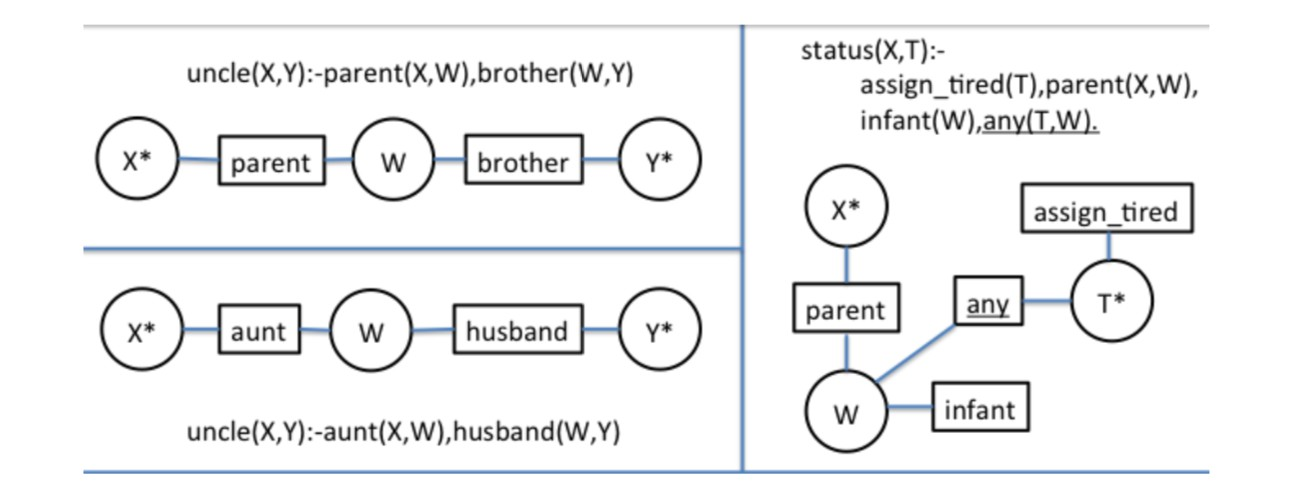
\includegraphics[width=10.25cm, height=3.7cm]{tensorlog}
	\end{center}
\end{figure}
\begin{itemize}
	\item TensorLog converts rules $r \in \mathcal{T}$ into factor graphs $G_r$. 
	\item  A factor graph is like an undirected graphical model which explicitly represents factors as nodes.
	\item Predicate symbols become factors which have edges connected to logical variables which are the arguments of the predicate.
	\item The matrix of a factor node for predicate $p$ is exactly $\textbf{M}_p$.
\end{itemize}
\end{frame}

\begin{frame}[fragile]
\frametitle{TensorLog Factor Graphs II}
\begin{figure}
	\begin{center}
		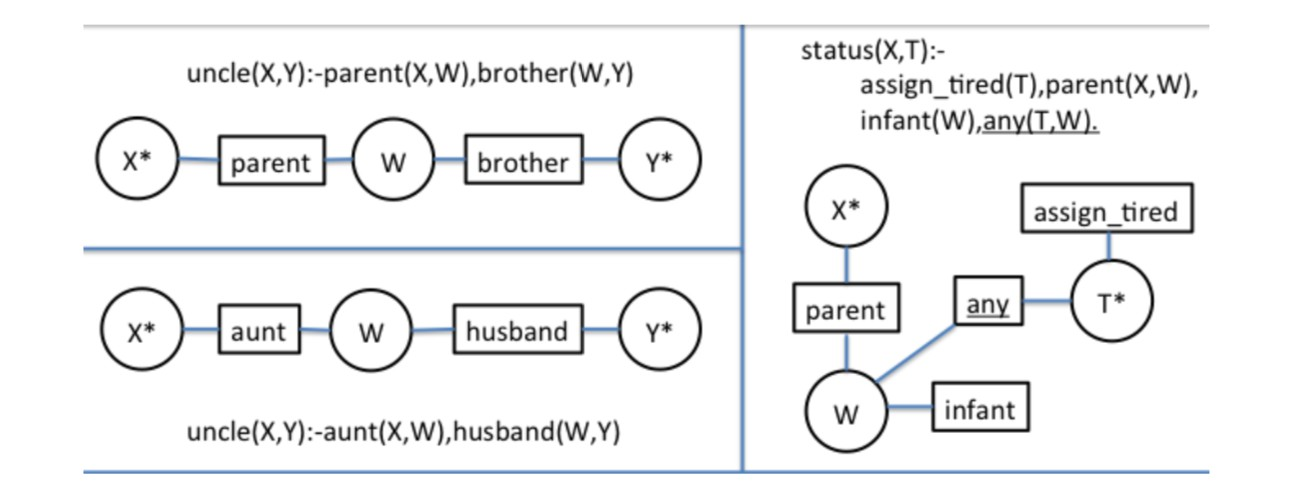
\includegraphics[width=11.25cm, height=4cm]{tensorlog}
	\end{center}
\end{figure}
\begin{itemize}
	\item Special \verb!any/2! and \verb!assign/1! predicates are introduced.
	\item  \verb!any/2! holds for any two constants in the language with probability 1.  It is used to connect disjoint factor graphs.
	\item \verb!assign/1! is a syntactic restriction which is ``algorithmically convenient".
\end{itemize}
\end{frame}

\begin{frame}[fragile]
\frametitle{TensorLog Inference I}
$G_r$ defines a distribution over possible groundings of the variables in $r$.  Let $X_1, ..., X_m$ be the variables in $r$.  Then:
\begin{gather*}
Pr_{G_r}(X_1 = c_1, ..., X_m = c_m) = \frac{1}{Z} \prod_{(c_i, c_j) \in E_r} \phi_r(c_i, c_j) = \prod_{(c_i, c_j) \in E_r} \theta_{r(c_i, c_j)}.
\end{gather*}
If $r(c_i, c_j) \notin \mathcal{DB}$ any substitution $r(X_i, X_j)\{X_i / c_i, X_j / c_j\}$ will have 0 probability.
\end{frame}

\begin{frame}[fragile]
\frametitle{TensorLog Inference II}
Assume that we are interested in the query \verb!uncle(c, Y)! for some $c \in C$.  We will perform BP over $G_{uncle}$ conditioned on $X = c$.  This corresponds to the following linear transformation:
\begin{gather*}
(\textbf{u}_c \textbf{M}_{parent})\textbf{M}_{brother}.
\end{gather*}
Recall that $\textbf{u}_c$ is a one-hot vector which encodes the position of the constant $c \in C$.  Then $\textbf{v}_W = \textbf{u}_c \textbf{M}_{parent}$ is a vector where $\textbf{v}_W[c'] = \theta_{parent(c, c')}$.  Finally $\textbf{v}_Y = \textbf{v}_W \textbf{M}_{brother}$ computes the marginal probability for $Y$ which is exactly what BP does in the message passing steps.
\end{frame}

\begin{frame}[fragile]
\frametitle{TensorLog Inference III}
\begin{itemize}
	\item BP in $G_r$ corresponds to simple linear transformations of the probability vector representations over $\mathcal{KB}$.
	\item In the case where some predicate is defined in multiple rules we simply return the sum of the response vectors for the individual definitions.
	\item For example, $g_{io}^{\verb!uncle!}(\textbf{u}_c) = g_{io}^{\verb!uncle!_1}(\textbf{u}_c) + g_{io}^{\verb!uncle!_2}(\textbf{u}_c)$ where $\verb!uncle!_i$ is the $ith$ definition for the predicate.
	\item If a predicate $r$ is defined by some $r' \in \mathcal{T}$ (as opposed to some $r' \in \mathcal{DB}$) we replace $\textbf{v}_{F, X} \leftarrow \textbf{v}_i \textbf{M}_r$ with $\textbf{v}_{F, X} \leftarrow g_{io}^{r'}(\textbf{v}_i)$ in compileMessage($F \rightarrow X$).
\end{itemize}
\end{frame}

\begin{frame}[fragile]
\frametitle{TensorLog BP Algorithm}
	\begin{algorithm}[H]
		\Fn{compileMessage$(F \rightarrow X)$: }{
			
			\KwData{
				Factor $F$ representing $r(X)$ or $r(X_i, X_o)$, \\
				\hspace*{1.15cm} Random variable $X$ representing the logical variable
			}
			\KwResult{Message from $F$ to $X$: $\textbf{v}_{F, X}$\newline}
			\uIf{$F = r(X)$}{
				$\textbf{v}_{F, X} \leftarrow \textbf{v}_r$
			}
			\uElseIf{$X$ is the output variable $X_o$ of $F$}{
				$\textbf{v}_i \leftarrow \text{compileMessage}(X_i \rightarrow F)$\\
				$\textbf{v}_{F, X} \leftarrow \textbf{v}_i \textbf{M}_r$
			}
			\ElseIf{$X$ is the input variable $X_i$ of $F$}{
				$\textbf{v}_o \leftarrow \text{compileMessage}(X_o \rightarrow F)$\\
				$\textbf{v}_{F, X} \leftarrow \textbf{v}_o \textbf{M}_{r}^{\top}$
			}
			\textbf{return} $\textbf{v}_{F, X}$
		}
	\end{algorithm}
\end{frame}

\begin{frame}[fragile]
\frametitle{TensorLog BP Algorithm}

\begin{algorithm}[H]
	\Fn{compileMessage$(X \rightarrow F)$: }{
		
		\KwData{
			Random variable $X$ representing the logical variable, \\
			\hspace*{1.15cm} Factor $F$ representing $r(X)$ or $r(X_i, X_o)$
		}
		\KwResult{Message from $X$ to $F$: $\textbf{v}_{X, F}$\newline}
		
		\uIf{$X$ is the given variable to the query}{
			$\textbf{v}_{X, F} \leftarrow \textbf{u}_c$ // return the one-hot vector
		}
		// if the only factor which has $X$ as an argument is $F$:\\
		\uElseIf{$\eta(X) = \{F\}$}{
			$\textbf{v}_{X, F} \leftarrow \textbf{1}$  // return a vector of all 1's
		}
		\Else{
			// loop over all $k$ of $X$'s neighbor literals $F_i$ except $F$\\
			\ForEach{$F_i \in \eta(X)\setminus F$}{
				$\textbf{v}_i \leftarrow \text{compileMessage}(F_i \rightarrow X)$
			}
			$\textbf{v}_{X, F} \leftarrow \textbf{v}_1 \circ ... \circ  \textbf{v}_k$ // $\circ$ is the element-wise product
		}
		\textbf{return} $\textbf{v}_{X, F}$
	}
\end{algorithm}
\end{frame}

\begin{frame}
\frametitle{Agenda}
\begin{itemize}
	\item Deep Learning
	\item Logical Student-Teacher Network
	\item Probabilistic Logic Programming
	\item TensorLog
	\item \textbf{Conclusion}
\end{itemize}
\end{frame}


\end{document}
